\documentclass[11pt,a4paper]{article}
\usepackage[margin=1in]{geometry}
\usepackage[T1]{fontenc}
\usepackage[utf8]{inputenc}
\usepackage{lmodern}
\usepackage{microtype}
\usepackage{booktabs}
\usepackage{array}
\usepackage{tabularx}
\usepackage{hyperref}
\usepackage{enumitem}
\usepackage{float}
\usepackage{titlesec}
\usepackage{xcolor}
\usepackage{tikz}
\usetikzlibrary{shapes.geometric, arrows.meta, positioning, fit, calc, backgrounds, shadows}

\definecolor{primary}{RGB}{30, 60, 114}     % Dark navy
\definecolor{secondary}{RGB}{42, 82, 152}   % Lighter navy
\definecolor{accent}{RGB}{0, 150, 136}      % Teal
\definecolor{lightbg}{RGB}{248, 249, 250}   % Very light gray
\definecolor{bordercol}{RGB}{200, 205, 210} % Soft border
\definecolor{textcol}{RGB}{51, 51, 51}

\hypersetup{
  colorlinks=true,
  linkcolor=primary,
  urlcolor=accent,
  citecolor=primary
}

\renewcommand{\familydefault}{\sfdefault}
\color{textcol}

\setlist[itemize]{leftmargin=1.8em, itemsep=2pt, topsep=4pt}
\setlist[enumerate]{leftmargin=1.8em, itemsep=2pt, topsep=4pt}
\titleformat{\section}{\Large\bfseries\color{primary}}{\thesection.}{0.5em}{}
\titleformat{\subsection}{\large\bfseries\color{secondary}}{\thesubsection.}{0.5em}{}
\titleformat{\subsubsection}{\normalsize\bfseries\color{secondary}}{\thesubsubsection.}{0.5em}{}

\title{\Huge\bfseries\color{primary} Technical Report\\[0.5ex] \Large Agentic Workflow for Automated Binary Analysis}
\author{}
\date{\today}

\begin{document}
\maketitle
\vspace{-3em}

\begin{abstract}
\noindent This report documents the implementation of a static binary analysis system for PE and ELF files. The system combines five specialized analyzers, a deterministic report generator, and an optional LLM-based orchestrator. The report explains the architecture, main design choices, evaluation results, operational usage, current limitations, and future work. The writing focuses on implementation and observed behavior rather than promotional description.
\end{abstract}

\section{Introduction}
The project targets automated malware triage for executable binaries. Its objective is to inspect a file, extract security-relevant indicators, and present the results in forms that are useful for both automated processing and human analysis. To meet this objective, the implementation uses two complementary paths:

\begin{itemize}
\item A \textbf{deterministic path} that always produces machine-readable and human-readable reports.
\item An \textbf{agentic path} that uses a Gemini-based orchestrator to generate a narrative summary from real tool outputs.
\end{itemize}

This separation is important. The deterministic path provides reproducibility and stable artifacts, while the agentic path improves readability for an analyst. The project is therefore designed as a layered system rather than as a single monolithic script.

\section{System Overview}
\subsection{Functional Scope}
The system supports the following main functions:

\begin{itemize}
\item validation of the input binary file;
\item parsing of PE and ELF metadata;
\item extraction of imports, sections, hashes, and architecture information;
\item detection of cryptographic constants and suspicious entropy patterns;
\item extraction of suspicious strings such as URLs, IP addresses, commands, and keywords;
\item analysis of imports and system-call related behavior;
\item detection of packing and obfuscation indicators, including an automatic unpack attempt for known packers;
\item generation of JSON and Markdown reports;
\item optional orchestration of tool calls through an LLM.
\end{itemize}

\subsection{High-Level Architecture}
The project follows a modular architecture with four main layers. This structure simplifies maintenance and helps separate concerns between parsing, analysis, orchestration, and output generation.

\begin{figure}[H]
\centering
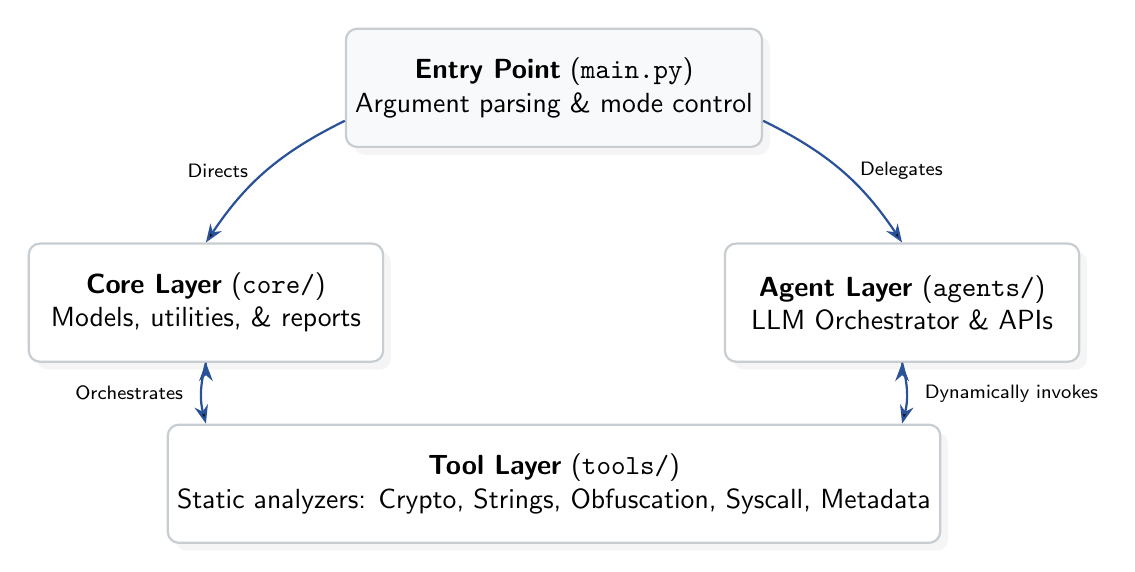
\begin{tikzpicture}[
    node distance=1.5cm and 1.5cm,
    layer/.style={draw=bordercol, thick, rounded corners, fill=white, minimum width=4.5cm, minimum height=1.5cm, align=center, font=\sffamily, drop shadow={opacity=0.08, shadow xshift=1mm, shadow yshift=-1mm}},
    arrow/.style={thick, ->, >=Stealth, draw=secondary},
    sublabel/.style={font=\sffamily\scriptsize\color{secondary}}
]

\node[layer, fill=lightbg] (entry) {\textbf{Entry Point} (\texttt{main.py}) \\ \sublabel{Argument parsing \& mode control}};

\node[layer, below left=1.2cm and -0.5cm of entry] (core) {\textbf{Core Layer} (\texttt{core/}) \\ \sublabel{Models, utilities, \& reports}};

\node[layer, below right=1.2cm and -0.5cm of entry] (agent) {\textbf{Agent Layer} (\texttt{agents/}) \\ \sublabel{LLM Orchestrator \& APIs}};

\node[layer, below=3.5cm of entry, minimum width=9.5cm] (tool) {\textbf{Tool Layer} (\texttt{tools/}) \\ \sublabel{Static analyzers: Crypto, Strings, Obfuscation, Syscall, Metadata}};

\draw[arrow] (entry) edge[bend right=15] node[left, font=\scriptsize\sffamily, xshift=-0.1cm] {Directs} (core.north);
\draw[arrow] (entry) edge[bend left=15] node[right, font=\scriptsize\sffamily, xshift=0.1cm] {Delegates} (agent.north);
\draw[arrow] (core.south) edge[bend right=15] node[left, font=\scriptsize\sffamily, xshift=-0.1cm] {Orchestrates} (tool.north -| core.south);
\draw[arrow] (agent.south) edge[bend left=15] node[right, font=\scriptsize\sffamily, xshift=0.1cm] {Dynamically invokes} (tool.north -| agent.south);

\end{tikzpicture}
\caption{Overall System Architecture and Layer Dependencies}
\label{fig:arch}
\end{figure}

\begin{table}[H]
\centering
\renewcommand{\arraystretch}{1.3}
\begin{tabularx}{\textwidth}{>{\bfseries\color{primary}}p{2.5cm} X}
\toprule
Layer & Role \\
\midrule
Entry point & Parses arguments, validates user choices, runs the selected mode, and saves generated reports. \\
Core layer & Defines shared data structures, binary loading helpers, file validation, entropy computation, and deterministic report aggregation. \\
Tool layer & Contains five analyzers, each focused on one aspect of malware triage. \\
Agent layer & Exposes tool wrappers to the Gemini-based orchestrator and produces a narrative report from real tool outputs. \\
\bottomrule
\end{tabularx}
\caption{Details on High-level project architecture layers}
\end{table}

\section{Technical Implementation Details}
\subsection{Entry Point and Execution Control}
The main entry point is implemented in \texttt{main.py}. It receives a binary path and selects one of three modes: \texttt{deterministic}, \texttt{agent}, or \texttt{both}. This file is responsible for the overall workflow.

\begin{figure}[H]
\centering
\begin{tikzpicture}[
    node distance=1cm and 2cm,
    step/.style={draw=bordercol, thick, rectangle, rounded corners, fill=white, minimum width=3.5cm, minimum height=0.8cm, align=center, font=\sffamily\footnotesize, drop shadow={opacity=0.08, shadow xshift=1mm, shadow yshift=-1mm}},
    decision/.style={draw=accent, thick, diamond, fill=lightbg, aspect=2, align=center, font=\sffamily\scriptsize, drop shadow={opacity=0.08, shadow xshift=1mm, shadow yshift=-1mm}, inner sep=0pt},
    arrow/.style={thick, ->, >=Stealth, draw=primary, rounded corners},
    label/.style={font=\sffamily\scriptsize, color=primary}
]

\node[step, fill=lightbg] (start) {\textbf{Initialize} \\ \scriptsize User Input \& Mode};
\node[decision, below=0.8cm of start] (isdet) {Deterministic \\ Mode?};
\node[step, right=1.5cm of isdet] (rundet) {Execute Core \\ Analyzers};
\node[step, below=0.6cm of rundet] (gendet) {Generate MD/JSON \\ Reports};

\node[decision, below=1.5cm of isdet] (isag) {Agent \\ Mode?};
\node[step, right=1.5cm of isag] (runag) {LLM Dynamically \\ Calls Tools};
\node[step, below=0.6cm of runag] (genag) {Stream Narrative \\ Output};

\node[step, fill=lightbg, below=0.8cm of isag] (end) {\textbf{Terminate}};

\draw[arrow] (start) -- (isdet);
\draw[arrow] (isdet) -- node[above, label] {Yes} (rundet);
\draw[arrow] (isdet) -- node[right, label] {No} (isag);
\draw[arrow] (rundet) -- (gendet);
\draw[arrow] (gendet) |- (isag);

\draw[arrow] (isag) -- node[above, label] {Yes} (runag);
\draw[arrow] (isag) -- node[right, label] {No} (end);
\draw[arrow] (runag) -- (genag);
\draw[arrow] (genag) |- (end);

\end{tikzpicture}
\caption{Workflow Control Flow}
\label{fig:workflow}
\end{figure}

In deterministic mode, the program runs the obfuscation detector first. This is a deliberate design choice because unpacking, if successful, should change the target file used by later analyzers. The resulting analysis target is then passed to metadata, crypto, string, and syscall analysis. After all tool outputs are collected, the deterministic report generator merges them into a single report and writes both JSON and Markdown artifacts to the output directory.

In agent mode, the program creates the orchestrator and asks it to inspect the target binary by calling the available tools. The agent output is printed directly to the terminal instead of being written as a structured report file.

In \texttt{both} mode, deterministic analysis is executed first and agent mode follows. This sequence is sensible because deterministic artifacts are more stable and can exist even if the LLM path fails or is skipped.

\subsection{Shared Data Model}
The project uses a shared schema defined in the core layer. This is one of the strongest implementation decisions in the codebase because all tools return results with a compatible structure. The main model entities are:

\begin{itemize}
\item \texttt{BinaryInfo}, which stores file-level metadata such as path, format, hashes, size, architecture, entry point, section list, and imports;
\item \texttt{SectionInfo}, which stores per-section properties including size, entropy, offsets, and permissions;
\item \texttt{ImportInfo}, which represents one imported function;
\item \texttt{Finding}, which represents one security-relevant observation with category, description, severity, confidence, ATT\&CK mapping, location, and details;
\item \texttt{AnalysisResult}, which represents the output of one analysis tool.
\end{itemize}

This common schema improves consistency in two ways. First, the deterministic report generator can aggregate tool outputs without format-specific special cases. Second, the agent layer can serialize tool outputs as JSON without inventing a new structure for each tool.

\subsection{Binary Parsing and Utility Layer}
The utility layer centralizes low-level binary processing. It validates the input file, rejects missing or empty files, and enforces a size limit of 100 MB. This protects the workflow from obvious misuse and avoids unnecessarily large inputs.

Format detection is based on magic bytes. PE files are identified from the \texttt{MZ} header and ELF files from the \texttt{0x7F ELF} magic. After format detection, the system computes MD5 and SHA-256 hashes and creates an initial \texttt{BinaryInfo} object.

Format-specific parsing is then applied:

\begin{itemize}
\item PE parsing uses \texttt{pefile} to read architecture, bitness, entry point, sections, permissions, and imports.
\item ELF parsing uses \texttt{pyelftools} to read architecture, bitness, entry point, sections, flags, and unresolved external symbols.
\end{itemize}

The utility layer also provides Shannon entropy calculation. This value is used later by analyzers to detect suspicious sections, encrypted blobs, and packing-related patterns.

\subsection{Tool Layer}
\subsubsection{Metadata Extractor}
The metadata extractor is responsible for the base structural description of the binary. Its output is important because it anchors later interpretations. A file cannot be meaningfully assessed without knowing its format, architecture, size, imported functions, and section properties. In practice, this analyzer provides the reference binary metadata used by the aggregated report.

\subsubsection{Crypto Detector}
The crypto detector searches for known cryptographic constants, crypto-related indicators, and entropy-based patterns. The design here is heuristic rather than semantic. The tool does not attempt to prove that a binary implements a specific algorithm in a full formal sense. Instead, it detects recognizable constants and suspicious patterns that often indicate encryption, hashing, or obfuscation. This is appropriate for triage because the goal is fast prioritization rather than full reverse engineering.

\subsubsection{String Analyzer}
The string analyzer extracts printable strings and classifies suspicious values. This tool is highly useful in malware triage because many indicators are directly visible as embedded strings. The implementation searches for URLs, IP addresses, shell commands, registry paths, file paths, and malware-related keywords. In the observed evaluation results, this analyzer produced the strongest tool score for the suspicious sample, which is consistent with its design.

\subsubsection{Syscall Analyzer}
The syscall analyzer maps imported functions and APIs to behavioral categories and ATT\&CK techniques. This tool provides a bridge between static imports and higher-level behavior. In simple binaries, its findings may be limited because import tables are sometimes small or uninformative. However, the design is still sound because it gives structured behavior hints without requiring execution of the sample.

\subsubsection{Obfuscation Detector}
The obfuscation detector searches for packer markers, entropy anomalies, import-table anomalies, overlay data, and anti-analysis indicators. This tool also contains the automatic unpacking logic. Its implementation detects packer names from section names and byte signatures. If a known packer is found and automatic unpacking is enabled, the detector attempts to create an unpacked copy of the sample and returns the path of the unpacked file when successful.

This design is especially important because packed binaries often reduce the usefulness of metadata, strings, and import analysis. For this reason, the deterministic workflow calls the obfuscation detector first.

\subsection{Deterministic Report Generator}
The deterministic report generator is implemented in the core layer. It collects outputs from all tools and produces a unified report with:

\begin{itemize}
\item generation timestamp;
\item original input file path;
\item binary metadata;
\item aggregated risk score;
\item per-tool risk scores;
\item severity counts;
\item deduplicated top findings;
\item ATT\&CK mappings;
\item operational recommendations;
\item raw tool results.
\end{itemize}

Two implementation details are especially relevant:

\begin{itemize}
\item Findings are deduplicated using category, description, ATT\&CK identifier, and location. This avoids repeated entries when more than one analyzer observes the same indicator.
\item The final risk score is computed as the average of the tool-level risk scores. This is simple, transparent, and reproducible, although it may not be the only possible scoring policy.
\end{itemize}

The report generator then produces a Markdown summary from the aggregated report. This gives the project a stable textual output even without the LLM.

\subsection{Agent Orchestrator}
The agent layer is implemented in \texttt{agents/orchestrator.py}. It exposes plain typed wrapper functions for each tool and then registers them with the Agno agent. The use of plain wrapper functions is a good design choice because it avoids metadata problems that can appear when decorators alter function signatures.

The system prompt imposes strong constraints on the model. It explicitly instructs the model to call every tool, avoid fabricating findings, and base conclusions only on real outputs. This is an appropriate safety measure for security-related analysis.

The current implementation selects the Gemini model \texttt{gemini-2.5-flash-lite} via the orchestrator settings.

\subsection{Runtime and Containerization}
The runtime is supported in Docker through three key files (\texttt{Dockerfile}, \texttt{docker-compose.yml}, \texttt{start.sh}).
The Docker image installs Python, build tools, binary utilities, parsing dependencies, and a pinned UPX release. It also compiles the sample C binaries during image build and switches execution to a non-root user. This is a good operational decision because it reduces friction for demonstrations and improves runtime hygiene.

The startup script checks for required Python modules, whether \texttt{upx} is available, and enforces loading environment variables from a local \texttt{.env} file automatically. This improves local and container usability.

\section{Evaluation Results}
\subsection{Evaluation Method}
The evaluation used two sources of evidence:

\begin{itemize}
\item the automated test suite included in the repository;
\item the generated analysis reports available in the \texttt{reports/} directory.
\end{itemize}

This is a practical evaluation method because it reflects both code-level correctness checks and end-to-end outputs from real sample binaries.

\subsection{Automated Test Results}
The project includes tests for utility functions, report generation, smoke execution of the five tools, and graceful handling of unpacking failure.

\begin{table}[H]
\centering
\renewcommand{\arraystretch}{1.3}
\begin{tabularx}{\textwidth}{>{\bfseries\color{primary}}p{4.4cm} X}
\toprule
Test Area & Observed Result \\
\midrule
Utility functions & Format detection, entropy calculation, and file validation are covered. \\
Report generation & Aggregation and Markdown rendering are covered. \\
Tool smoke checks & All five tools are exercised on the sample binary. \\
Automatic unpacking & The unpacking path is tested for graceful failure when \texttt{upx} is unavailable. \\
\bottomrule
\end{tabularx}
\caption{Current test coverage}
\end{table}

\subsection{Deterministic Analysis Outputs}
Two deterministic outputs were available for inspection: one for \texttt{samples/fake\_malware} and one for \texttt{samples/mock}.

\begin{table}[H]
\centering
\renewcommand{\arraystretch}{1.3}
\begin{tabular}{p{4.2cm} p{2cm} p{2cm} p{3.3cm}}
\toprule
\textbf{\color{primary}Sample} & \textbf{\color{primary}Risk Score} & \textbf{\color{primary}Findings} & \textbf{\color{primary}Artifacts} \\
\midrule
\texttt{fake\_malware} & 36.0 & 35 & JSON and Markdown generated \\
\texttt{mock} & 3.0 & 1 & JSON and Markdown generated \\
\bottomrule
\end{tabular}
\caption{Observed deterministic report outputs}
\end{table}

The \texttt{fake\_malware} sample produced a richer output with 1 critical, 7 high, 19 medium, and 8 low findings. The per-tool risk scores were:

\begin{table}[H]
\centering
\renewcommand{\arraystretch}{1.3}
\begin{tabular}{p{5.4cm} p{2.4cm}}
\toprule
\textbf{\color{primary}Tool} & \textbf{\color{primary}Risk Score} \\
\midrule
Metadata extractor & 0.0 \\
Crypto detector & 45.0 \\
String analyzer & 100.0 \\
Syscall analyzer & 0.0 \\
Obfuscation detector & 35.0 \\
\bottomrule
\end{tabular}
\caption{Per-tool scores for the \texttt{fake\_malware} sample}
\end{table}

These values are coherent with the sample characteristics. The strongest signals came from suspicious strings, cryptographic constants, and packing indicators. By contrast, metadata and syscall analysis produced weaker signals for this file.

\section{How to Run and Use the Project Correctly}
\subsection{Prerequisites}
The project can be run locally with Python 3.11+ or inside Docker. The recommended path is Docker because it packages the parsing libraries and the UPX dependency in a controlled environment.
Agent mode requires a valid \texttt{GOOGLE\_API\_KEY} stored in a local \texttt{.env} file.

\subsection{Recommended Docker Procedure}
The correct steps are:

\begin{enumerate}
\item Build the image with \texttt{docker compose build}.
\item Run deterministic analysis with\\
\texttt{docker compose run --rm analysis ./start.sh samples/fake\_malware --mode deterministic}
\item Run agent analysis with\\
\texttt{docker compose run --rm analysis ./start.sh samples/fake\_malware --mode agent}
\item Run both paths with\\
\texttt{docker compose run --rm analysis ./start.sh samples/fake\_malware --mode both}
\item Add \texttt{--auto-unpack} when analyzing a packed sample.
\end{enumerate}

\subsection{Mode Selection}
\begin{table}[H]
\centering
\renewcommand{\arraystretch}{1.3}
\begin{tabularx}{\textwidth}{>{\bfseries\color{primary}}p{4.5cm} X}
\toprule
Need & Recommended Mode \\
\midrule
Stable report files for submission or grading & \texttt{deterministic} \\
Narrative explanation for an analyst & \texttt{agent} \\
Complete run with saved reports and terminal summary & \texttt{both} \\
Packed sample investigation & \texttt{deterministic} or \texttt{both} with \texttt{--auto-unpack} \\
\bottomrule
\end{tabularx}
\caption{Recommended mode selection}
\end{table}

For most reliable use, \texttt{deterministic} mode should be treated as the primary execution path because it always creates reproducible artifacts.

\section{Conclusions}
The project is well structured and implements the main components required for automated static malware triage. The strongest part of the system is the deterministic path. It is modular, reproducible, and based on a clear shared data model. The Docker workflow is also well chosen because it reduces setup friction and packages native dependencies.

The architecture demonstrates good separation of concerns. The core layer provides reusable binary parsing and reporting logic, the tool layer keeps each analysis task focused, and the agent layer adds an optional interpretation interface.

The evaluation results show that the project is functional in practice. It produces reports correctly for the inspected samples and the automated tests cover important parts of the implementation.

\section{Future Work}
The following improvements would provide the highest value:

\begin{itemize}
\item integrate automatic unpacking into the full end-to-end workflow so that the agent path can reuse the unpacked artifact when available;
\item improve the unpacking subsystem with better diagnostics, explicit UPX error reporting, and support for more packers;
\item make the test suite more robust across platforms by controlling temporary directories and avoiding host-specific permission failures;
\item add evaluation on a larger and more diverse sample set to measure false positives, false negatives, and consistency of scoring;
\item save the agent output to a file so that both execution paths produce persistent artifacts;
\item refine risk aggregation with a weighting scheme that reflects the relative strength of different analyzers;
\item enrich ATT\&CK mapping and add clearer explanation for why a finding maps to a given technique.
\end{itemize}

\section{References}
\begin{enumerate}
\item Agno documentation and Python package for agent-based tool orchestration.
\item FastMCP documentation for exposing Python functions as tool interfaces.
\item \texttt{pefile} documentation for Portable Executable parsing in Python.
\item \texttt{pyelftools} documentation for ELF parsing in Python.
\item MITRE ATT\&CK framework, used for technique mapping in findings.
\item UPX documentation, used for automatic unpacking support in the Docker image.
\item Project source files.
\end{enumerate}

\end{document}
